\section{}

% remarque : pour qu'un mot se retrouve dans le lexique : \MotDefinition{asymptote horizontale}{} 

\begin{methode*1}[Savoir utiliser le vocabulaire]

\begin{aconnaitre}[Nombres relatifs]
Un \MotDefinition{nombre relatif positif}{} s'écrit avec le signe $+$ ou sans signe.

Un \MotDefinition{nombre relatif négatif}{} s'écrit avec le signe $-$. 

0 est le seul nombre à la fois positif et négatif.

Deux nombres relatifs qui ne diffèrent \textbf{que} par leur signe sont \textbf{opposés}.
\end{aconnaitre}

\begin{exemple*1}
Quel est le signe du nombre – 3 ? Quel est son opposé ? \\[1em]
Le signe de $- 3$ est $-$, il est négatif. Son opposé est $+ 3$ que l'on écrit aussi 3.
\end{exemple*1}

\exercice 
Donne le signe des nombres relatifs suivants :

$+ 1235$ ; $- 587$ ; 0 ; $- 1$ ;  3,5 ; $- 0,001$.
%\correction

\exercice 
Donne l'opposé des nombres relatifs suivants :

$- 2\,531$ ; 0 ; 1\,245 ;  $- 0,03$ et 0,003.
%\correction

\end{methode*1}

%%%%%%%%%%%%%%%%%%%%%%%%%%%%%%%%%%%%%%%%%%%%%%%%%%%%%%%%%%%%%%%%%

\begin{methode*1}[Repérer un point sur une droite graduée]

\begin{aconnaitre}
Tout point d'une droite graduée est repéré par un nombre relatif appelé son \MotDefinition{abscisse}{}.
\end{aconnaitre}

\begin{center} 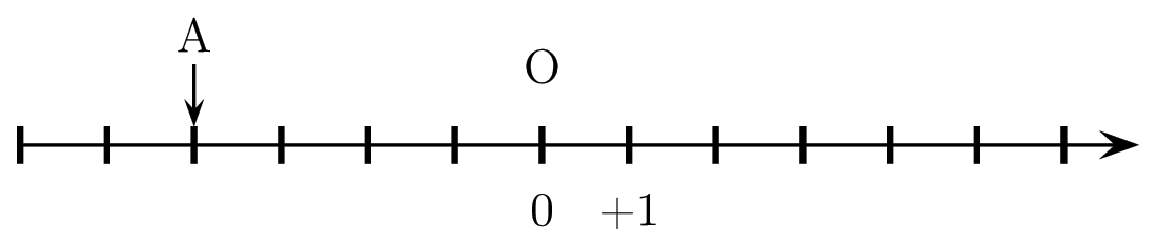
\includegraphics[width=8.5cm]{axeAO} \end{center}

\begin{exemple*1}
Sur la droite graduée ci-dessus, lis l'abscisse du point $A$ : \\[1em]
\begin{minipage}[c]{0.4\linewidth}
Le point $A$ est à gauche de l'origine :

son abscisse est donc négative.

La distance du point $A$ au point $O$ est 4.
 \end{minipage} \hfill%
 \begin{minipage}[c]{0.1\linewidth}
 \begin{center}
\includegraphics[width=0.23cm]{accolade_droite}\end{center}
  \end{minipage} \hfill%
  \begin{minipage}[c]{0.4\linewidth}
  donc l'abscisse du point $A$ est $- 4$.
   \end{minipage} \\
\end{exemple*1}


\begin{exemple*1}
Trace une droite graduée et place les points $B(+ 6)$ et $C(- 5)$ : \\[1em]
\begin{minipage}[c]{0.4\linewidth}
L'abscisse du point $B$ est $+ 6$ donc
 \end{minipage} \hfill%
 \begin{minipage}[c]{0.1\linewidth}
 \begin{center}
\includegraphics[width=0.23cm]{accolade_gauche}\end{center}
  \end{minipage} \hfill%
  \begin{minipage}[c]{0.4\linewidth}
  Son abscisse est positive : le point $B$ est donc à droite de l'origine.
  
  Sa distance à l'origine est de 6 unités.
  \end{minipage} \\[0.5em]

\begin{minipage}[c]{0.4\linewidth}
L'abscisse du point $C$ est $- 5$ donc
 \end{minipage} \hfill%
 \begin{minipage}[c]{0.1\linewidth}
 \begin{center}
\includegraphics[width=0.23cm]{accolade_gauche}\end{center}
  \end{minipage} \hfill%
  \begin{minipage}[c]{0.4\linewidth}
  Son abscisse est négative : le point $C$ est donc à gauche de l'origine. 
  
  Sa distance à l'origine est de 5 unités.
   \end{minipage} \\
\begin{center} 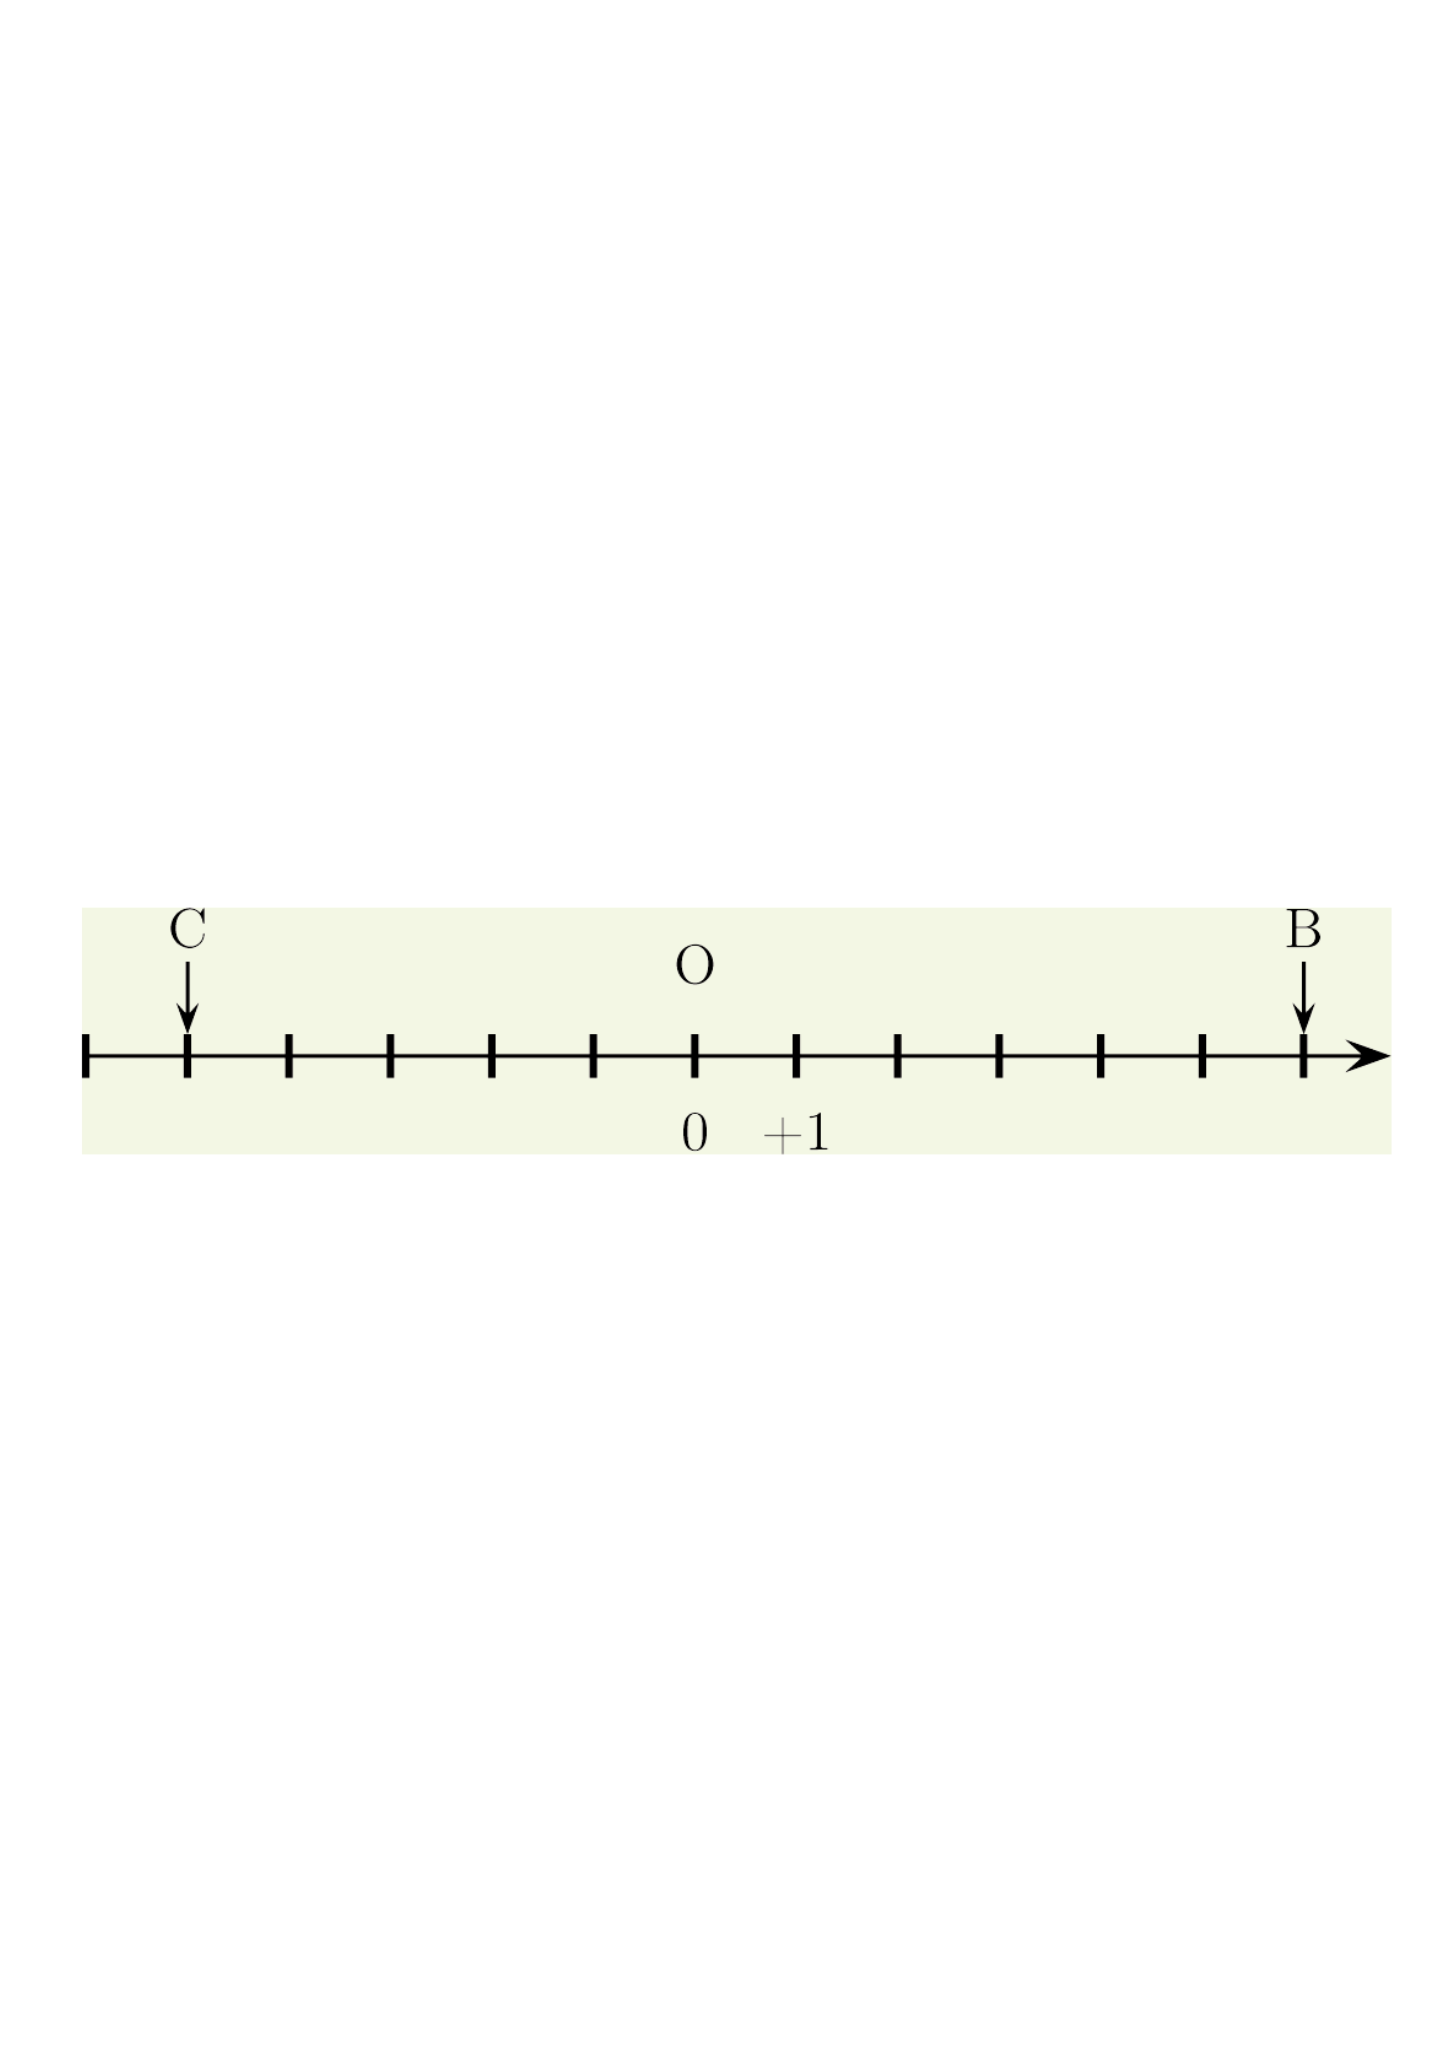
\includegraphics[width=8.5cm]{axeCOB} \end{center}
\end{exemple*1}


\exercice
Trace une droite graduée d'origine $O$, une unité valant 2 cm. Places-y les points $A$, $B$, $C$, $D$ et  $E$, $F$ d'abscisses respectives $+ 3$ ; $- 2$ ; $+ 5$ ; $- 3$ et $- 1,5$ ; $+ 2,5$. Que peux-tu dire des abscisses de $A$ et $D$ ?
%\correction

\end{methode*1}


%%%%%%%%%%%%%%%%%%%%%%%%%%%%%%%%%%%%%%%%%%%%%%%%%%%%%%%%%%%%%%%%%

\begin{methode*1}[Trouver la valeur absolue d'un nombre relatif]

\begin{aconnaitre}
La \MotDefinition{valeur absolue}{} d'un nombre relatif est le nombre sans son signe.

Sur une droite graduée, cela correspond à la distance entre l'origine et le point qui a pour abscisse ce nombre.
\end{aconnaitre}

\begin{exemple*1}
Donne la valeur absolue du nombre $- 2$ :

La valeur absolue du nombre $- 2$ est 2.
\end{exemple*1}


\exercice
Donne la valeur absolue des nombres suivants : $+ 5$ ; $- 7$ ; $+ 64,78$ et $- 123,4$.
%\correction

\end{methode*1}


%%%%%%%%%%%%%%%%%%%%%%%%%%%%%%%%%%%%%%%%%%%%%%%%%%%%%%%%%%%%%%%%%

\begin{methode*1}[Repérer un point dans un plan]

\begin{aconnaitre}
Dans un plan muni d'un repère, tout point est repéré par un couple de nombres relatifs appelé ses \MotDefinition{coordonnées}{} : la première est l'\textbf{abscisse} et la seconde est l'\MotDefinition{ordonnée}{}.
\end{aconnaitre}

\begin{exemple*1}
Lis les coordonnées du point $A$ et du point $B$ :
\begin{center} 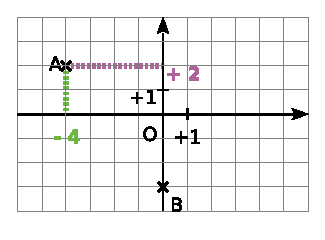
\includegraphics[width=4.7cm]{grapheAOB} \end{center}

Pour lire les coordonnées du point $A$, on repère l'abscisse de $A$ sur l'axe horizontal puis  son ordonnée sur l'axe vertical. On conclut en donnant l'abscisse puis l'ordonnée : $A (- 4 ; + 2)$. \\[0.5em]
Le point $B$ appartient à l'axe des ordonnées donc son abscisse est 0. Ses coordonnées sont $(0 ; - 3)$.
\end{exemple*1}

\begin{exemple*1}
Dans un repère place les points $C(5 ; - 3)$ et $D(- 4 ; 0)$ : \\[0.5cm]
\begin{center} 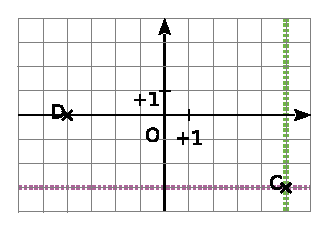
\includegraphics[width=3.7cm]{grapheDOC} \end{center}
\vspace{0.5cm}
Pour placer le point $C$, on repère tous les points d'abscisse $+ 5$ (ligne verte) puis on repère tous les points d'ordonnée $- 3$ (ligne violette). On place le point $C$ à l'intersection des deux lignes. \\[0.5em]
L'ordonnée du point $D$ est 0 donc le point $D$ appartient à l'axe des abscisses.
\end{exemple*1}

\exercice % J'ai déplacé cet ex. car sinon on sort de la section exemple.
\begin{minipage}[c]{0.45\linewidth}
Sur la figure ci-dessous, lis les coordonnées des points $K$, $L$, $M$, $N$, $P$ et $R$ :
 \end{minipage} \hfill%
 \begin{minipage}[c]{0.4\linewidth}
 \vspace{2cm}
 \begin{center} 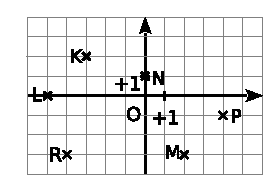
\includegraphics[width=3.8cm]{grapheKRM} \end{center}
  \end{minipage} \\
%\correction

\exercice Trace sur ton cahier un repère d'origine $O$. L'unité de longueur est le centimètre sur les deux axes. Place les points suivants :
\begin{colenumerate}{4}
 \item $E(+ 2 ; + 3)$ ;
 \item $F(- 2 ; - 3)$ ;
 \item $G(+ 2 ; - 3)$ ;
 \item $H(- 2 ; 3)$.
 \end{colenumerate}
%\correction

\end{methode*1}


%%%%%%%%%%%%%%%%%%%%%%%%%%%%%%%%%%%%%%%%%%%%%%%%%%%%%%%%%%%%%%%%%

\begin{methode*1}[Comparer deux nombres relatifs]

\begin{aconnaitre}
\MotDefinition{Comparer deux nombres}{}, c'est trouver lequel est le plus grand (ou le plus petit) ou dire s'ils sont égaux.
\end{aconnaitre}

\begin{exemple*1}
Compare 9,37 et 92,751 puis 81,36 et 81,357 :

On compare d'abord les \textbf{\textcolor{H1}{parties entières}} des deux nombres :
\begin{itemize}
 \item $\textbf{\textcolor{H1}{9}} < \textbf{\textcolor{H1}{92}}$ donc $9,37 < 92,751$.
 \item 81,357 et 81,36 ont la même partie entière. On compare alors les \textbf{\textcolor{B2}{parties décimales}} : $81,357 = 81 + 0,357$ et $81,36 = 81 + 0,36$ mais $0,36 = 0,360$.
 \end{itemize}
Or \textbf{\textcolor{B2}{360 millièmes}} est plus grand que \textbf{\textcolor{B2}{357 millièmes}} donc 81,36 > 81,357.
\end{exemple*1}


\begin{exemple*1}
Écris un encadrement de 1,564 au dixième : \\[0.5em]
$1,564 = 1+ 0,500 + 0,064$ et 0,064 est plus petit que 1 dixième. Ainsi, 1,564 est compris entre $1 + 0,5$ et $1 + 0,5 + 0,1$ , soit $1 + 0,6$. \\[0.5em]
Donc un encadrement au dixième de 1,564 est : $1,5 < 1,564 < 1,6$.
\end{exemple*1}

\begin{aconnaitre}
\textbf{Deux nombres relatifs positifs} sont rangés dans l'ordre de leur valeur absolue.

Un \textbf{nombre relatif négatif} est inférieur à un \textbf{nombre relatif positif}.

\textbf{Deux nombres relatifs négatifs} sont rangés dans l'ordre inverse de leur valeur absolue.
\end{aconnaitre}

\begin{exemple*1}
Compare les nombres $- 9$ et $- 7$ : \\[0.5em]
\begin{tabular}{ccl} 
 $- 9$ et $- 7$ & $\longrightarrow$ & On veut comparer deux nombres relatifs négatifs. \\
 $9 \textcolor{H1}{>} 7$ & $\longrightarrow$ & On détermine les valeurs absolues de $- 9$ et de $- 7$ puis on les compare. \\
 $- 9 \textcolor{H1}{<} - 7$ & $\longrightarrow$ & On range les nombres $- 9$ et $- 7$ dans l'ordre inverse de leur valeur absolue. \\
 \end{tabular}
\end{exemple*1}


\exercice
Compare les nombres suivants :
\begin{colenumerate}{3}
 \item $+ 5$ et $+ 9$ ;
 \item $- 3$ et $+ 8$ ;
 \item $- 6$ et $- 12$ ;
 \item $- 5$ et $- 9$ ;
 \item 5,1 et $- 5,3$ ;
 \item $- 6,2$ et $- 6,4$.
 \end{colenumerate}
%\correction

\exercice
Range dans l'ordre croissant les nombres suivants : 
\begin{colenumerate}{2}
 \item $+ 12$ ; 0 ; $- 7$ ; $- 5$ ; $+ 5$ ;
 \item $- 8$ ; $+ 10$ ; $- 14$ ; $- 21$ ; $+ 3$ ; $- 1$ ;
 \item $- 24$ ; $- 2,4$ ; 2,4 ; 0 ; $- 4,2$ ; $- 4$ ;
 \item $- 2,4$ ; $+ 2,3$ ; $- 2,42$ ; $+ 2,33$ ; $- 3,23$.
 \end{colenumerate}
%\correction

\end{methode*1}

